\usepackage[utf8]{inputenc}
\usepackage[english,russian]{babel}
\usepackage[14pt]{extsizes}

%\usepackage{pscyr}
\usepackage{subfigure}
\usepackage{wrapfig}
\usepackage{cmap}
\usepackage{indentfirst}
\usepackage{autonum}
\usepackage{amsfonts}
\usepackage{amsmath}
\usepackage{amssymb}
\usepackage{amsthm}
\usepackage{upgreek}
\usepackage{graphicx}
\usepackage{listings}
\usepackage{multirow}
\usepackage{multicol}
\usepackage{dsfont}
\usepackage{graphicx}
\usepackage{caption}
\usepackage{setspace,amsmath}

\usepackage[unicode, pdftex]{hyperref}
\usepackage[left=30mm, top=20mm, right=15mm, bottom=20mm, footskip=10mm]{geometry}
\usepackage{xcolor}

\definecolor{maroon}{cmyk}{0, 0.87, 0.68, 0.32}
\definecolor{halfgray}{gray}{0.55}
\definecolor{ipython_frame}{RGB}{207, 207, 207}
\definecolor{ipython_bg}{RGB}{247, 247, 247}
\definecolor{ipython_red}{RGB}{186, 33, 33}
\definecolor{ipython_green}{RGB}{0, 128, 0}
\definecolor{ipython_cyan}{RGB}{64, 128, 128}
\definecolor{ipython_purple}{RGB}{170, 34, 255}

\usepackage{listings}
\lstset{
    breaklines=true,
    texcl=true,
    %
    extendedchars=true,
    literate=
    {á}{{\'a}}1 {é}{{\'e}}1 {í}{{\'i}}1 {ó}{{\'o}}1 {ú}{{\'u}}1
    {Á}{{\'A}}1 {É}{{\'E}}1 {Í}{{\'I}}1 {Ó}{{\'O}}1 {Ú}{{\'U}}1
    {à}{{\`a}}1 {è}{{\`e}}1 {ì}{{\`i}}1 {ò}{{\`o}}1 {ù}{{\`u}}1
    {À}{{\`A}}1 {È}{{\'E}}1 {Ì}{{\`I}}1 {Ò}{{\`O}}1 {Ù}{{\`U}}1
    {ä}{{\"a}}1 {ë}{{\"e}}1 {ï}{{\"i}}1 {ö}{{\"o}}1 {ü}{{\"u}}1
    {Ä}{{\"A}}1 {Ë}{{\"E}}1 {Ï}{{\"I}}1 {Ö}{{\"O}}1 {Ü}{{\"U}}1
    {â}{{\^a}}1 {ê}{{\^e}}1 {î}{{\^i}}1 {ô}{{\^o}}1 {û}{{\^u}}1
    {Â}{{\^A}}1 {Ê}{{\^E}}1 {Î}{{\^I}}1 {Ô}{{\^O}}1 {Û}{{\^U}}1
    {œ}{{\oe}}1 {Œ}{{\OE}}1 {æ}{{\ae}}1 {Æ}{{\AE}}1 {ß}{{\ss}}1
    {ç}{{\c c}}1 {Ç}{{\c C}}1 {ø}{{\o}}1 {å}{{\r a}}1 {Å}{{\r A}}1
    {€}{{\EUR}}1 {£}{{\pounds}}1
}

%%
%% Python definition (c) 1998 Michael Weber
%% Additional definitions (2013) Alexis Dimitriadis
%% modified by me (should not have empty lines)
%%
\lstdefinelanguage{iPython}{
    morekeywords={access,and,break,class,continue,def,del,elif,else,except,exec,finally,for,from,global,if,import,in,is,lambda,not,or,pass,print,raise,return,try,while},%
    %
    % Built-ins
    morekeywords=[2]{abs,all,any,basestring,bin,bool,bytearray,callable,chr,classmethod,cmp,compile,complex,delattr,dict,dir,divmod,enumerate,eval,execfile,file,filter,float,format,frozenset,getattr,globals,hasattr,hash,help,hex,id,input,int,isinstance,issubclass,iter,len,list,locals,long,map,max,memoryview,min,next,object,oct,open,ord,pow,property,range,raw_input,reduce,reload,repr,reversed,round,set,setattr,slice,sorted,staticmethod,str,sum,super,tuple,type,unichr,unicode,vars,xrange,zip,apply,buffer,coerce,intern},%
    %
    sensitive=true,%
    morecomment=[l]\#,%
    morestring=[b]',%
    morestring=[b]",%
    %
    morestring=[s]{'''}{'''},% used for documentation text (mulitiline strings)
    morestring=[s]{"""}{"""},% added by Philipp Matthias Hahn
    %
    morestring=[s]{r'}{'},% `raw' strings
    morestring=[s]{r"}{"},%
    morestring=[s]{r'''}{'''},%
    morestring=[s]{r"""}{"""},%
    morestring=[s]{u'}{'},% unicode strings
    morestring=[s]{u"}{"},%
    morestring=[s]{u'''}{'''},%
    morestring=[s]{u"""}{"""},%
    %
    % {replace}{replacement}{lenght of replace}
    % *{-}{-}{1} will not replace in comments and so on
    literate=
    {á}{{\'a}}1 {é}{{\'e}}1 {í}{{\'i}}1 {ó}{{\'o}}1 {ú}{{\'u}}1
    {Á}{{\'A}}1 {É}{{\'E}}1 {Í}{{\'I}}1 {Ó}{{\'O}}1 {Ú}{{\'U}}1
    {à}{{\`a}}1 {è}{{\`e}}1 {ì}{{\`i}}1 {ò}{{\`o}}1 {ù}{{\`u}}1
    {À}{{\`A}}1 {È}{{\'E}}1 {Ì}{{\`I}}1 {Ò}{{\`O}}1 {Ù}{{\`U}}1
    {ä}{{\"a}}1 {ë}{{\"e}}1 {ï}{{\"i}}1 {ö}{{\"o}}1 {ü}{{\"u}}1
    {Ä}{{\"A}}1 {Ë}{{\"E}}1 {Ï}{{\"I}}1 {Ö}{{\"O}}1 {Ü}{{\"U}}1
    {â}{{\^a}}1 {ê}{{\^e}}1 {î}{{\^i}}1 {ô}{{\^o}}1 {û}{{\^u}}1
    {Â}{{\^A}}1 {Ê}{{\^E}}1 {Î}{{\^I}}1 {Ô}{{\^O}}1 {Û}{{\^U}}1
    {œ}{{\oe}}1 {Œ}{{\OE}}1 {æ}{{\ae}}1 {Æ}{{\AE}}1 {ß}{{\ss}}1
    {ç}{{\c c}}1 {Ç}{{\c C}}1 {ø}{{\o}}1 {å}{{\r a}}1 {Å}{{\r A}}1
    {€}{{\EUR}}1 {£}{{\pounds}}1,
    %
    literate=
    *{+}{{{\color{ipython_purple}+}}}1
    {-}{{{\color{ipython_purple}-}}}1
    {*}{{{\color{ipython_purple}$^\ast$}}}1
    {/}{{{\color{ipython_purple}/}}}1
    {^}{{{\color{ipython_purple}\^{}}}}1
    {?}{{{\color{ipython_purple}?}}}1
    {!}{{{\color{ipython_purple}!}}}1
    {\%}{{{\color{ipython_purple}\%}}}1
    {<}{{{\color{ipython_purple}<}}}1
    {>}{{{\color{ipython_purple}>}}}1
    {|}{{{\color{ipython_purple}|}}}1
    {\&}{{{\color{ipython_purple}\&}}}1
    {~}{{{\color{ipython_purple}~}}}1
    %
    {==}{{{\color{ipython_purple}==}}}2
    {<=}{{{\color{ipython_purple}<=}}}2
    {>=}{{{\color{ipython_purple}>=}}}2
    %
    {+=}{{{+=}}}2
    {-=}{{{-=}}}2
    {*=}{{{$^\ast$=}}}2
    {/=}{{{/=}}}2,
    %
    commentstyle=\color{ipython_cyan}\ttfamily,
    stringstyle=\color{ipython_red}\ttfamily,
    keepspaces=true,
    showspaces=false,
    showstringspaces=false,
    rulecolor=\color{ipython_frame},
    frame=single,
    frameround={t}{t}{t}{t},
    framexleftmargin=6mm,
    numbers=left,
    numberstyle=\tiny\color{halfgray},
    %
    backgroundcolor=\color{ipython_bg},
    % extendedchars=true,
    basicstyle=\scriptsize\ttfamily,
    keywordstyle=\color{ipython_green}\ttfamily,
    escapechar=\%,
    escapebegin=\color{ipython_green},
    texcl=true,
    inputencoding=utf8
}

\begin{document}
	\selectlanguage{russian}
\setcounter{page}{0}

\begin{center}
	\small{Министерство науки и высшего образования Российской Федерации}\\
	\small{Федеральное государственное бюджетное образовательное учреждение}\\
	\small{Высшего образования}\\
	\small{\textbf{«Северо-Осетинский государственный университет\\
			имени Коста Левановича Хетагурова»}}\\
	
	\hfill \break
	\hfill \break
	\hfill \break
	\hfill \break
	\hfill \break
	\hfill \break
	\hfill \break
	\hfill \break
	\hfill \break
	\hfill \break
	\hfill \break
	\hfill \break
	\hfill \break
	
	\normalsize{Дипломная работа}\\
	\large{\textbf{Seq2Seq - подход для реализации машинного перевода}}\\
	
	\hfill \break
	\hfill \break
	\hfill \break
	\hfill \break
	\hfill \break
	\hfill\break
\end{center}

\begin{flushright}
	\textbf{Выполнил:}\\
	Студент 4 курса направления:\\
	«Прикладная математика и информатика»\\
	\textit{Гамосов Cтанислав Станиславович \underline{\hspace{3cm}}}\\
\end{flushright}

\hfill

\begin{flushright}
	\textbf{Научный руководитель:}\\
	Кандидат физико-математических наук:\\
	\textit{Басаева Елена Казбековна \underline{\hspace{3cm}}}\\
\end{flushright}

\hfill

\begin{flushright}
	\textbf{Консультант}\\
	Старший преподаватель: \\
	\textit{Макаренко Мария Дмитриевна \underline{\hspace{3cm}}}\\
\end{flushright}

\normalsize{ \hspace{28pt}} \hfill \break
\begin{center} Владикавказ 2022 \end{center}
\thispagestyle{empty}
\clearpage
	\thispagestyle{empty}
\tableofcontents
\thispagestyle{empty}
\clearpage
\newtheorem{theorem}{Теорема}

	\begin{center}
	    \textbf{Аннотация}
	\end{center}
	
	В работе рассмотрена модель машинного перевода Seq2Seq c использованием нескольких архитектур рекуррентных нейронных сетей (LSTM и GRU). На практике полученные модели были хороши для работы с последовательностями, однако возникают трудности при запоминании долгосрочных зависимостей.
	
	\clearpage
	
	\section{Введение}
	
	В работе рассматривается задача машинного преревода на основе рекурентных нейронных сетей (RNN). Машинный перевод получил резкий скачек в качестве за последние годы из-за начала использования в них RNN. Они позволили снизить затраты на выявления лингвистических закономерностей языков и дорогостоящую разработку алгоритмов для их обработки. Статистический перевод хоть и не удалось полностью сместить, однако его количество в современных переводчиках снизилось почти до минимума. При построении хорошей модели машинного перевода необходимо учитывать внутреннюю структуру языка, семантику слов и связи между ними. В последние годы для решения этой проблемы часто используются (\cite{10}, \cite{11}, \cite{12}) модели sequence-to-sequence.
	
	Seq2Seq - это семейство подходов машинного обучения, используемых для обработки языка. Основные задачи в которых используется методы: нейронный перевод, субтитры к изображениям, разговорные модели и обобщение текста.
	
	Первоначальный алгоритм, который в процессе породил целое семейство методов, был разработан Google для использования в машинном переводе. Как уже можно заметить за последнюю пару лет коммерческие системы стали удивительно хороши в  переводе - посмотрите, например, Google Translate, Яндекс-Переводчик, переводчик DeepL, переводчик Bing Microsoft.
	
	Однако данная технология несет в себе огромный потенциал, помимо привычного машинного перевода между естественными языками, вполне реализуем перевод между языками программирования (Facebook AI - Глубокое обучение переводу между языками программирования). Поэтому возможности применений такого рода подходов довольно велики. В связи с этим под машинным переводом можно подразумевать любую задачу в переводе одной последовательности в любую другую.
	
	\clearpage
	
	\section{Рекуррентные сети}
	
	\subsection{RNN - Recиrrent Neural Network}
	
	\textit{Рекуррентные Нейронные Сети} (Recиrrent Neural Network - RNN) - это нелинейная динамическая система, которая сопоставляет последовательности с последовательностями. Основная философия заключается, в том что мысли обладают неким постоянством и напрямую зависят от прошлых умозаключений. 
	
	\begin{wrapfigure}{r}{0.25\textwidth}
		\centering
		\captionsetup{justification=centering}
		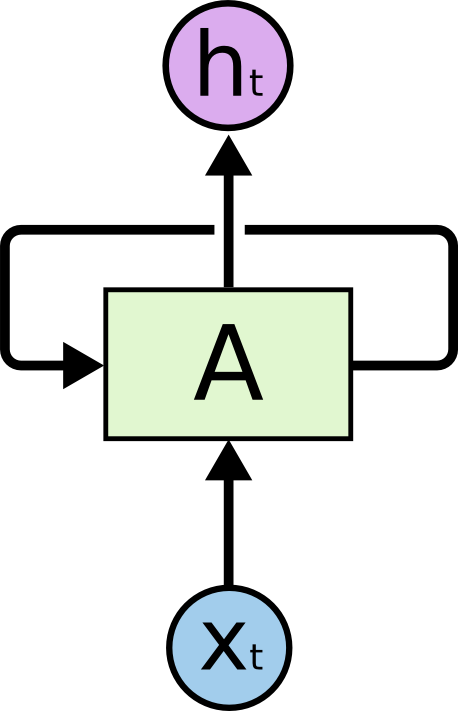
\includegraphics[height=45mm]{img/2.png}
		\caption{Рекуррентная нейронная сеть}
	\end{wrapfigure}
	
	RNN способны работать с последовательностями произвольной длины, а не с входными данными фиксированного размера. Это свойство как раз таки очень важно в контексте обработки естественных языков. Так же важное отличие таких сетей от обычных это понятие времени. Под ним подразумевается последовательность входных данных $x_t$, которая поступает на вход, и их выходная последовательность $y_t$, которые генерируются на основе дискретной входной последовательности. 
	
	Чтобы понять, что это значит, давайте проведем мысленный эксперимент. Скажем, вы делаете снимок шара, движущегося во времени.Допустим также, что вы хотите предсказать направление движения мяча. Таким образом, имея только ту информацию, которую вы видите на экране, как бы вы это сделали? Ну, вы можете пойти дальше и сделать предположение, но любой ответ, который вы придумали, был бы случайным предположением. Не зная, где находится мяч, у вас не будет достаточно данных, чтобы предсказать, куда он движется.Если вы запишете много снимков положения мяча подряд, у вас будет достаточно информации, чтобы сделать лучший прогноз.
	
	В результате получаемые последовательности могут быть конечной длины или бесконечно счетными. Таким образом, входную последовательность можно обозначить $x = (x_1, x_2, x_3, ... , x_t)$, а выходную последовательность как $y = (y_1, y_2, y_3, ... , y_t)$
	
	На схеме нейронная сеть $A$ принимает входное значение $x_t$ и возвращает значение $h_t$. Наличие обратной связи позволяет передавать информацию от одного шага сети к другому.
	
	Рекуррентную сеть можно рассматривать, как несколько копий одной и той же сети, каждая из которых передает информацию последующей копии. Вот, что произойдет, если мы развернем обратную связь:
	
	\begin{figure}[ht!]
		\centering
		\captionsetup{justification=centering}
		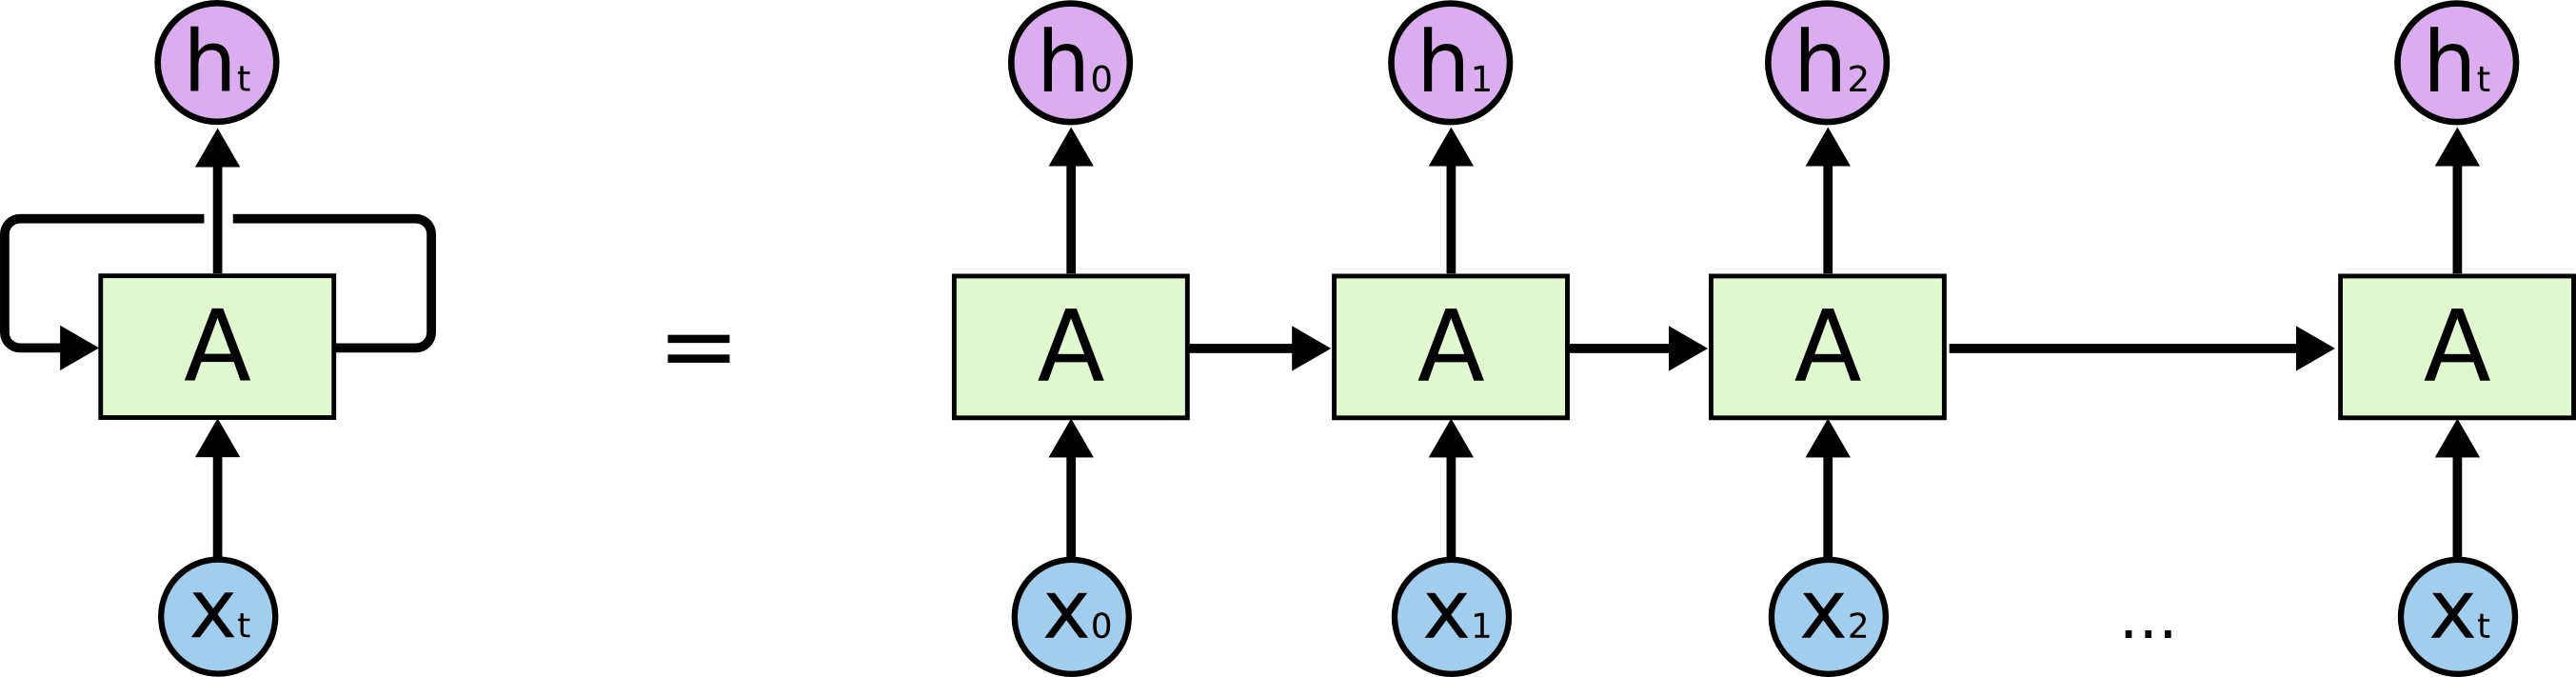
\includegraphics[height=40mm]{img/3.png}
		\caption{Развернутая рекуррентная нейронная сеть}
	\end{figure}
	
	То, что RNN напоминают цепи, может сказать нам лишь о том, что их довольно просто приложить к последовательностям. На данный этап RNN - самая естественная архитектура нейронных сетей для работы с данными таких типов.
	
	За последние несколько лет RNN с невероятным успехом применили к целому ряду задач: распознавание речи, языковое моделирование, распознавание изображений... Само собой в данной работе нас интересует, что такие сети довольно хорошо работают для задачи машинного перевода.
	
	\subsubsection{Elman Networks}
	
	Для большей понимания рекуррентных сетей рассмотрим, пару архитектур. Нейронная сеть Элмана состоит из трёх слоев: $x, y, h$. Дополнительно к сети добавлен набор \textit{контекстных блоков} - $c$. Скрытый слой $h$ соединён с контекстными блоками с фиксированным весом, равным единице. В данном случае веса равны единицам, однако это не всегда так. В свою очередь \textit{вес} - это связь между вершинами, которая несет в себе значение, характеризующее важность, передаваемого значения, проходящего через данное ребро. 
	
	Для пары узлов $i$ (узел входного слоя) и $j$ (узел скрытого слоя) присутствует собственный вес $w_{i,j}$. Легче всего это представить как матрицу смежности $W$, где на пересечение $i$ строки и $j$ столбца находятся числа отвечающие за вес. Такая же матрица только для скрытого слоя в выходной слой будем обозначать $U$. 
	
	С каждым шагом времени на вход $x$ поступает информация, которая проходит прямой ход к выходному слою $y_v$ в соответствии с правилами обучения. Фиксированные обратные связи сохраняют предыдущие значения скрытого слоя $h$ в контекстных блоках $c$ (до того как скрытый слой поменяет значение в процессе обучения). Таким способом сеть сохраняет своё состояние, что может использоваться в предсказании последовательностей, выходя за пределы мощности многослойного перцептрона.
	
	\begin{table}[h]
		\centering
		\begin{tabular}{|c|} 
			\hline
			\textbf{Elman Networks}  \\ 
			\hline
			$ h_{t} = \sigma_{h}(W_h x_t + U_h h_{t - 1} + b_h) $ \\ 
			$ y_{t} = \sigma_{y}(W_y h_t + b_y) $ \\
			\hline
		\end{tabular}
	\end{table}
	\begin{tabbing}
		$x_t$, $h_t$, $y_t$  - векторы входного, скрытого, выходного слоя        \\
		$W$, $U$ и $b$ - матрицы и вектор параметров       \\
		$\sigma_h$ и $\sigma_y$ - функции активации
	\end{tabbing}
	
	\textit{Функция активации} $\sigma$ в свою очередь является абстракцией, представляющей скорость возбуждения нейрона. Список функций активации, которых чаще всего используют:
	
	\begin{tabbing}
			\textit{Функция Хевисайда}:       &   
			$ H(x) = 
			\begin{cases}
				0, & x < 0 \\
				1, & x >= 0 \\
			\end{cases}$ \\ 
			\textit{Cигмоида}:                &  $\sigma(x) = \frac{1}{1 + e^{-x}}$ \\ 
			\textit{Гиперболический тангенс}: &  $tanh(x) = \frac{e^x - e^{-x}}{e^x + e^{-x}}$ \\ 
			\textit{Линейный выпрямитель}:    &  $ReLU(x) = max(0, x)$ \\
	\end{tabbing}

	\begin{tabbing}
	    Некоторые желательные свойства функций активации:\\
		\ \ \textit{Нелинейность} \\
		\ \ \textit{Непрерывная дифференцируемость} \\
		\ \ \textit{Ограниченность области значений} \\
		\ \ \textit{Монотонность} \\
		\ \ \textit{Гладкость функции с монотонной производной} \\
		\ \ \textit{Аппроксимировать тождественной функцию около начала координат} \\
	\end{tabbing}
	
	\subsubsection{Jordan Networks}
    
    Так же существует вторая архитектура RNN нейронная сеть Джордана. Подобна сети Элмана, но контекстные блоки связаны не со скрытым слоем, а с выходным слоем. Контекстные блоки таким образом сохраняют своё состояние. Они обладают рекуррентной связью с собой.
    
	\begin{table}[h]
			\centering
			\begin{tabular}{|c|} 
				\hline
				\textbf{Jordan Networks}  \\ 
				\hline
				$	h_{t} = \sigma_{h}(W_h x_t + U_h y_{t - 1} + b_h) $  \\
				$	y_{t} = \sigma_{y}(W_y h_t + b_y) $ \\
				\hline
			\end{tabular}
	\end{table}
	
	\begin{tabbing}
		$x_t$, $h_t$, $y_t$  - векторы входного, скрытого, выходного слоя        \\
		$W$, $U$ и $b$ - матрицы и вектор параметров       \\
		$\sigma_h$ и $\sigma_y$ - функции активации
	\end{tabbing}
	
	\begin{figure}[ht!]
		\centering
		\captionsetup{justification=centering}
		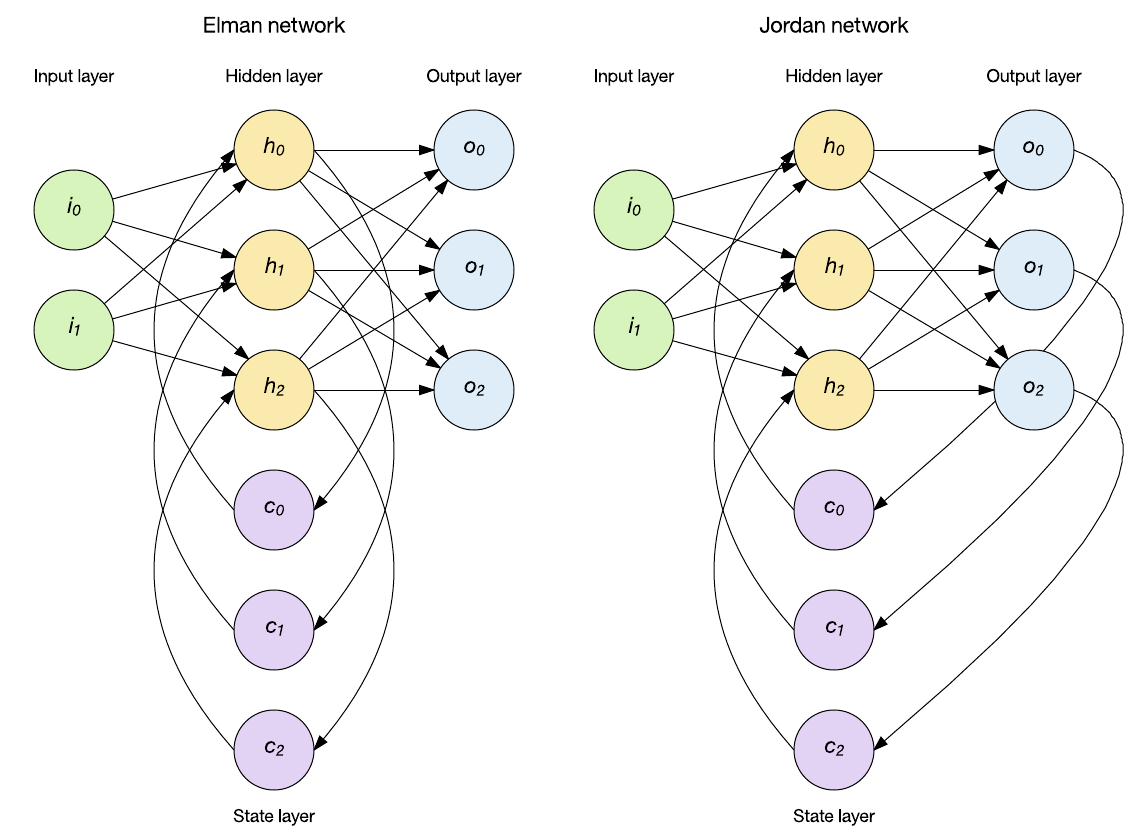
\includegraphics[width=140mm]{img/RNN.png}
		\caption{Схемы архиетектур рекуррентных нейронных сетей}
	\end{figure}
	
	\subsection{Проблема долговременных зависимостей}
	
	Одна из привлекательных идей RNN состоит в том, что они потенциально умеют связывать предыдущую информацию с текущей задачей. Как это было на примере полета шарика. Однако действительно ли RNN предоставляют нам такую возможность? Это зависит от некоторых обстоятельств.

	Во время работы с RNN было замечено, что случае, когда дистанция между актуальной информацией и местом, где она понадобилась, велика, то сети могут могут забыть нужную информацию из прошлого. Долгосрочные зависимости плохо воспринимаются обычными рекурсивными сетями, потому что градиенты имеют тенденцию либо исчезать (большую часть времени), либо взрываться (редко, но с серьезными последствиями). Это затрудняет метод оптимизации на основе градиента не только из-за различий в величинах градиента, но и из-за того, что эффект долгосрочных зависимостей скрыт эффектом краткосрочных зависимостей. 
	
	Существовало два доминирующих подхода, с помощью которых многие исследователи попытались уменьшить негативные последствия этой проблемы. Один из таких подходов заключается в разработке лучшего самообучающийся алгоритм, чем простой стохастический градиентный спуск.
	
	Другой подход, который нас больше интересует, заключается в разработке более сложной функции активации, чем обычные функции что применялись ранее. Самая ранняя попытка в этом направлении привела к появлению функции активации или повторяющегося блока, называемого блоком долговременной кратковременной памяти (LSTM)\cite{2}. Более современный тип повторяющейся единицы, к которому мы относимся как к закрытой повторяющейся единице (GRU)\cite{3}. Было показано, что некоторые из этих повторяющихся блоков хорошо справляются с задачами, требующими учета долгосрочных зависимостей.
	
	\subsection{GRNN - Gated Recurrent Neural Networks}
	\subsubsection{LSTM - Long Short-Term Memory}
	
	Сети долгой краткосрочной памяти (LSTM) - особая разновидность архитектуры RNN, способная к обучению долговременным зависимостям. Они были представлены Зеппом Хохрайтер и Юргеном Шмидхубером в 1997 \cite{2}. Они прекрасно решают целый ряд разнообразных задач и в настоящее время широко используются. Любая рекуррентная нейронная сеть имеет форму цепочки повторяющихся модулей нейронной сети. В обычной RNN структура одного такого модуля очень проста, например, он может представлять собой один слой с функцией активации $tanh$. 
	
	\begin{figure}[ht!]
		\centering
		\captionsetup{justification=centering}
		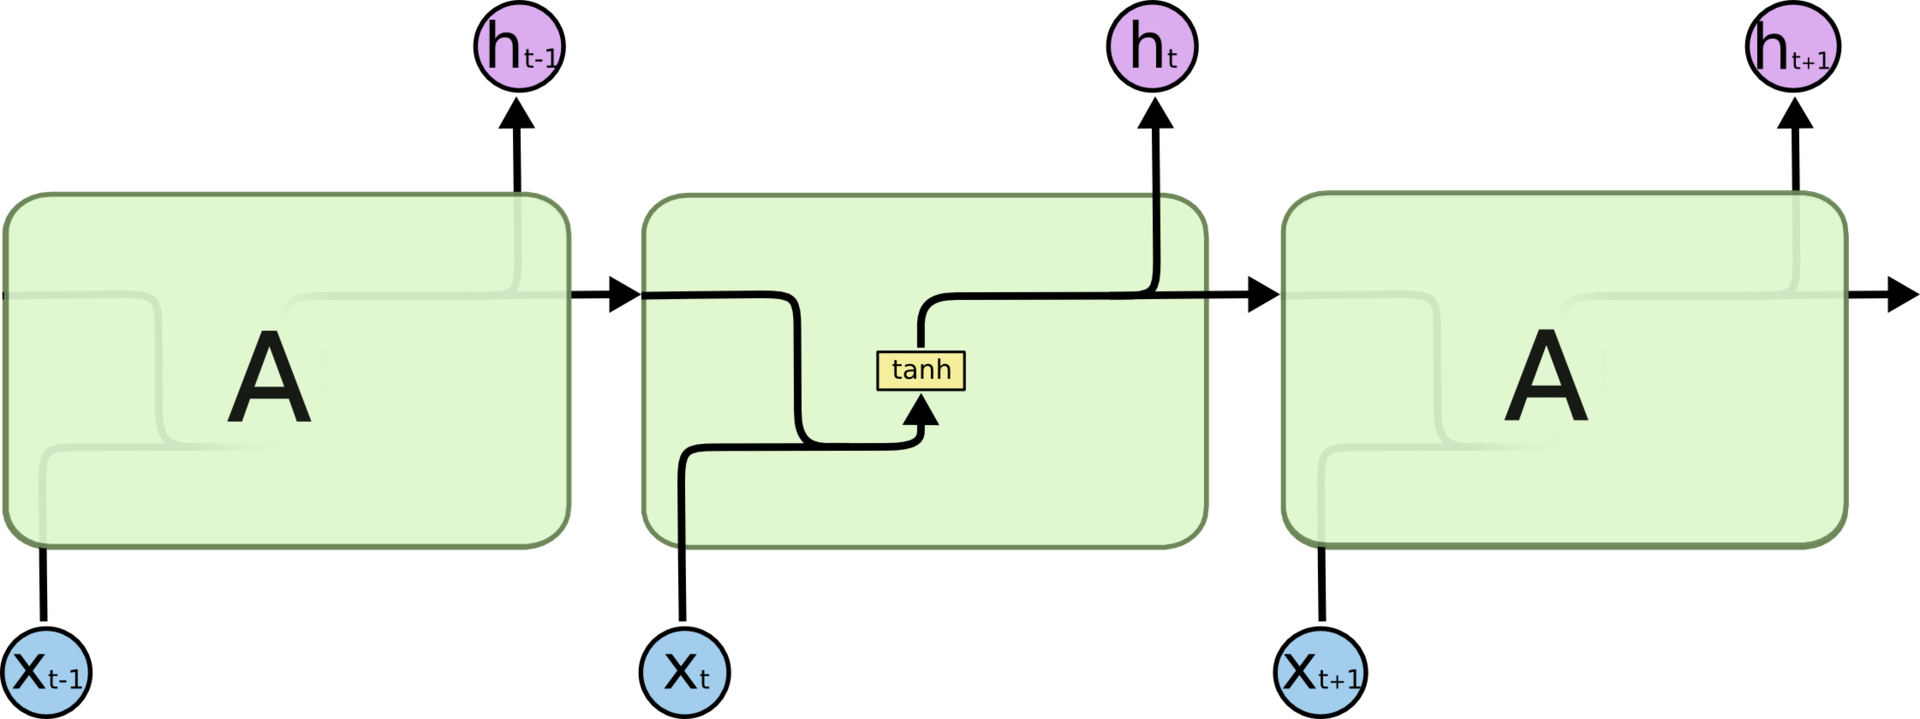
\includegraphics[height=40mm]{img/RNN Chain.png}
		\caption{Повторяющийся модуль в стандартной RNN состоит из одного слоя}
	\end{figure}
	
	Структура LSTM также напоминает цепочку, но модули выглядят иначе. Вместо одного слоя нейронной сети они содержат целых четыре, и эти слои взаимодействуют особенным образом. 
	
	\begin{figure}[ht!]
		\centering
		\captionsetup{justification=centering}
		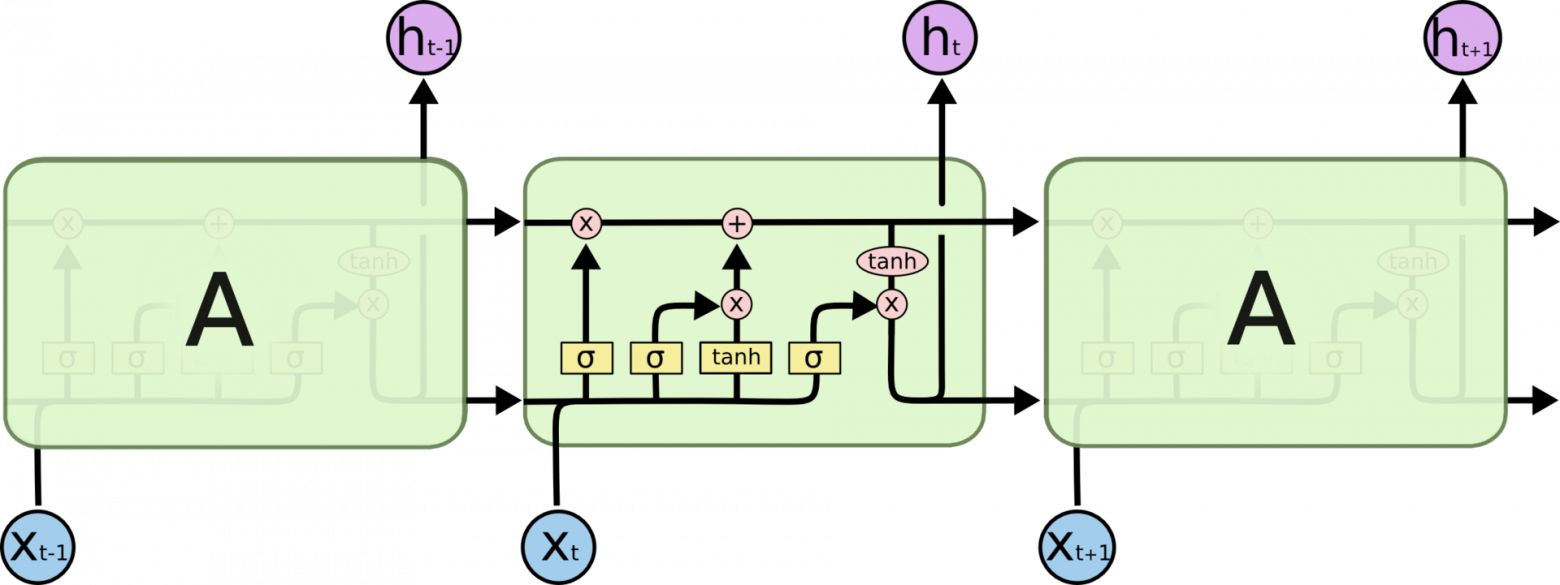
\includegraphics[height=40mm]{img/LSTM Chain.png}
		\caption{LSTM сети состоит из четырех взаимодействующих слоев}
	\end{figure}
	
	Ключевой компонент LSTM – это состояние ячейки (cell state) – горизонтальная линия, проходящая по верхней части схемы
	
	Состояние ячейки напоминает конвейерную ленту. Она проходит напрямую через всю цепочку, участвуя лишь в нескольких линейных преобразованиях. Информация может легко течь по ней, не подвергаясь изменениям.
	
	\begin{figure}[ht!]
		\centering
		\captionsetup{justification=centering}
		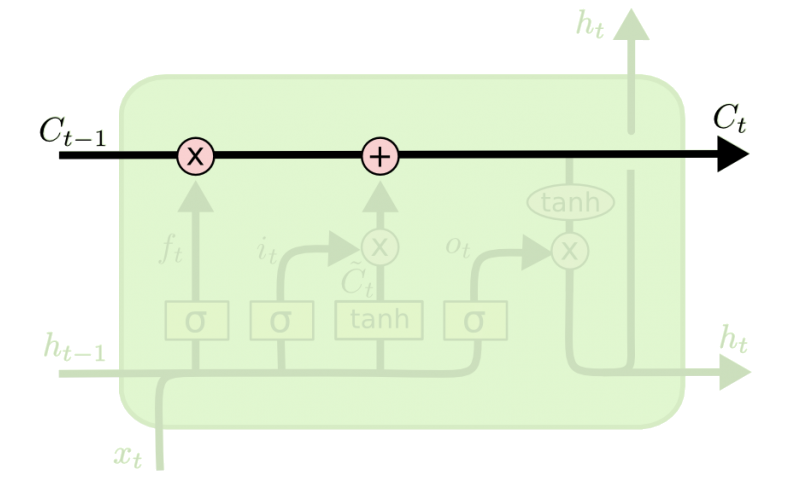
\includegraphics[height=40mm]{img/LSTM 1.png}
	\end{figure}
	
	Тем не менее, LSTM может удалять информацию из состояния ячейки; этот процесс регулируется структурами, называемыми фильтрами (gates). Фильтры позволяют пропускать информацию на основании некоторых условий. Они состоят из слоя сигмоидальной нейронной сети и операции поэлементного умножения.
	
	Сигмоидальный слой возвращает числа от нуля до единицы, которые обозначают, какую долю каждого блока информации следует пропустить дальше по сети. Ноль в данном случае означает \textit{не пропускать ничего}, единица - \textit{пропустить все}.

    \textit{Пошаговая работа LSTM:}
    
    Первый шаг в LSTM - определить, какую информацию можно выбросить из состояния ячейки. Это решение принимает слой на котором применяем сигмойду, называемый \textit{слоем фильтра забывания} (forget gate layer). Он смотрит на $h_{t-1}$ и $x_t$ и возвращает число от 0 до 1 для каждого числа из состояния ячейки $C_{t-1}$.
    
    \begin{figure}[ht!]
		\centering
		\captionsetup{justification=centering}
		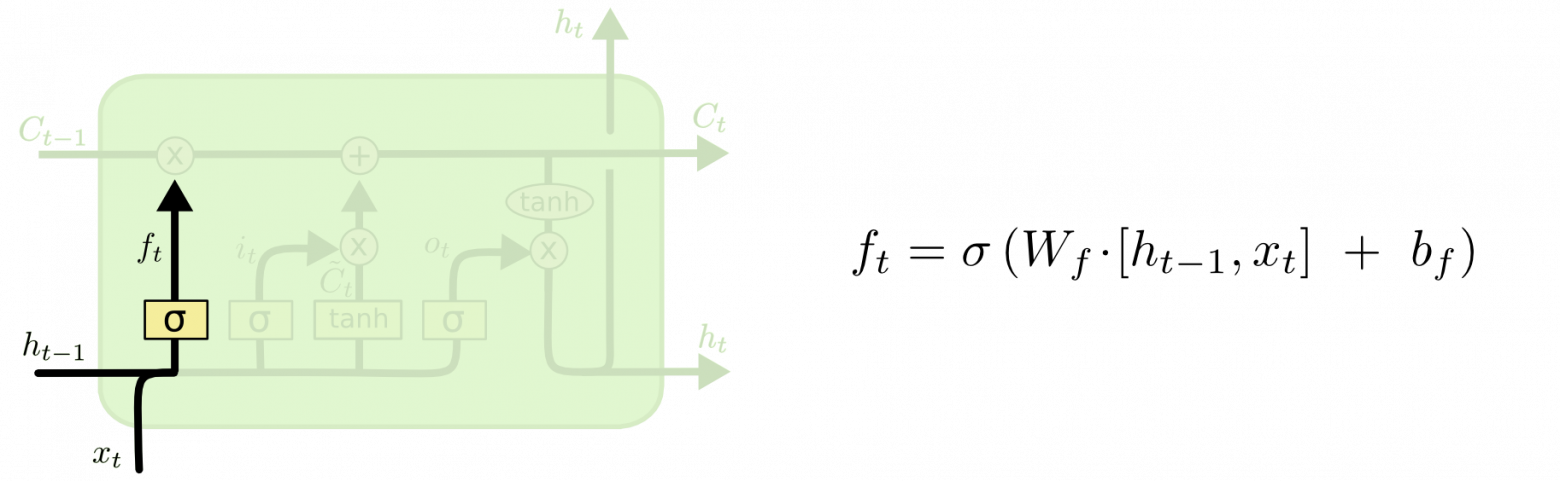
\includegraphics[height=40mm]{img/LSTM_step1.png}
	\end{figure}
	
	Следующий шаг - решить, какая новая информация будет храниться в состоянии ячейки. Этот этап состоит из двух частей. Сначала сигмоидальный слой под названием \textit{слой входного фильтра} (input layer gate) определяет, какие значения следует обновить. Затем действует функция активации tanh, в результате пролучаем вектор новых значений-кандидатов $\tilde{c}_t$, которые можно добавить в состояние ячейки.
    
    \begin{figure}[ht!]
		\centering
		\captionsetup{justification=centering}
		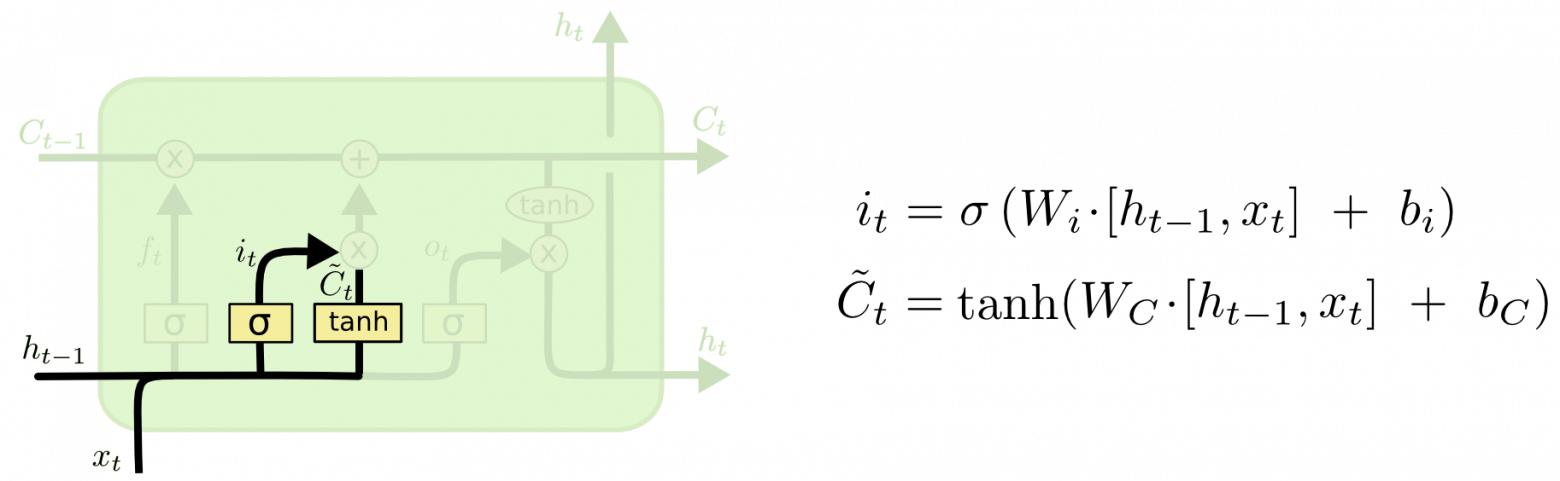
\includegraphics[height=40mm]{img/LSTM_step2.png}
	\end{figure}
	
    После всего этого нужно заменить старое состояние ячейки $c_{t-1}$ на новое состояние $c_t$.
    
    Необходимо умножить старое состояние на $f_t$, забывая то, что мы решили забыть. Затем прибавляем $i_t*\tilde{c}_t$. Это новые значения-кандидаты, умноженные на $t$ – на сколько мы хотим обновить каждое из значений состояния.
    
    \begin{figure}[ht!]
		\centering
		\captionsetup{justification=centering}
		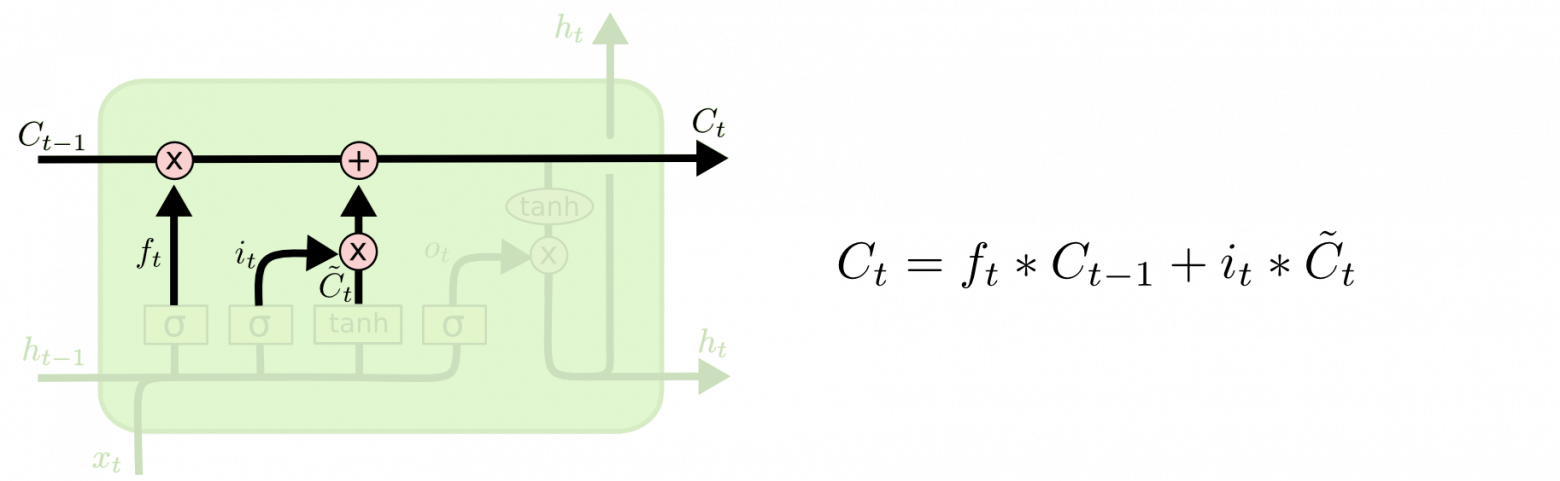
\includegraphics[height=40mm]{img/LSTM_step3.png}
	\end{figure}
	
	Наконец, нужно решить, какую информацию мы хотим получать на выходе. Выходные данные будут основаны на нашем состоянии ячейки, к ним будут применены некоторые фильтры. Сначала мы применяем функцию активации сигмойд, которая решает, какую информацию из состояния ячейки мы будем выводить. Затем значения состояния ячейки проходят через активацию tanh, чтобы получить на выходе значения из диапазона от -1 до 1, и перемножаются с выходными значениями сигмоидального слоя, что позволяет выводить только требуемую информацию.

    \begin{figure}[ht!]
		\centering
		\captionsetup{justification=centering}
		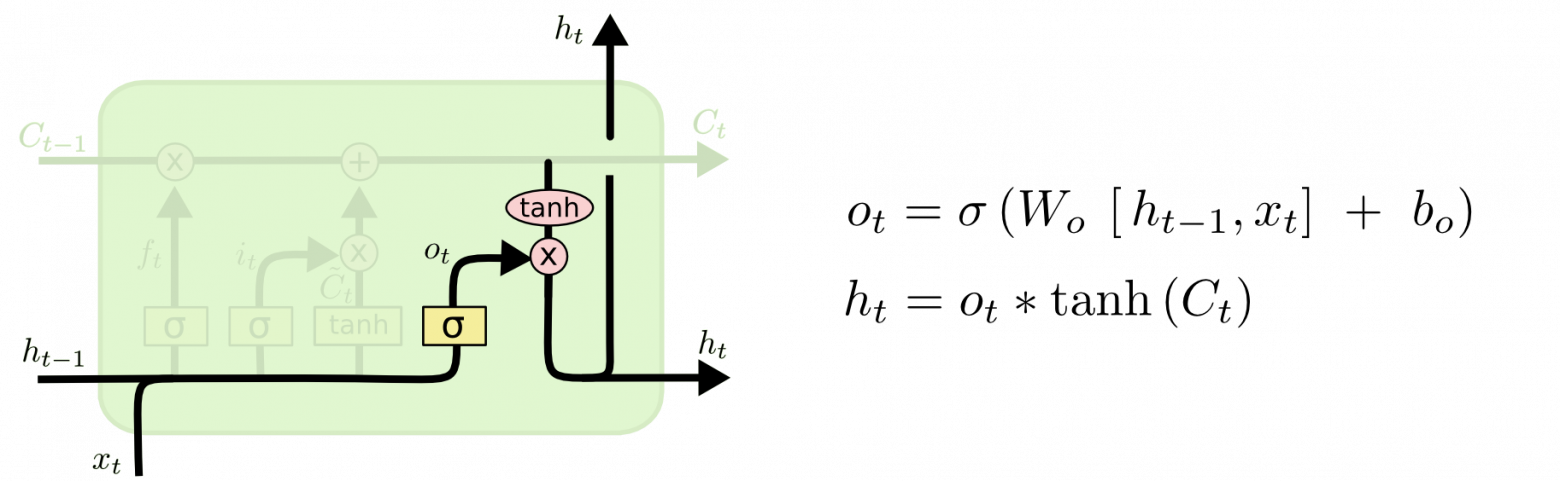
\includegraphics[height=40mm]{img/LSTM_step4.png}
	\end{figure}
	
	В отличие от традиционных рекуррентных сетей, которые перезаписывают свое содержимое на каждом шаге времени, блок LSTM способен решать, следует ли сохранять существующую память или нет с помощью введенных элементов. Интуитивно понятно, что если модуль LSTM обнаруживает важную функцию из входной последовательности на ранней стадии, он легко переносит эту информацию на большие расстояния, следовательно, фиксируя потенциальные зависимости.
	
	\subsubsection{GRU - Gated Recurrent Unit}
	
	Управляемые рекуррентные блоки была предложена в 2014 \cite{3}, чтобы каждая рекуррентная единица могла адаптивно фиксировать зависимости разных временных масштабов. Аналогично блоку LSTM, GRU имеет
	фильтра, которые модулируют поток информации внутри блока, однако, не имея отдельных ячеек памяти.
	
    GRU избавилось от ячеек состояния и использует скрытое состояние для передачи информации. Эта архитектура также имеет только два фильтра, фильтр сброса и фильтр обновления.
    
    \textit{Слой фильтра обновления} (update layer gate) элемент обновления действует аналогично слоям входного и выходного фильтра в LSTM. Он решает, какую информацию выбросить и какую новую информацию добавить.
    
    \textit{Слой фильтра сброса} (reset layer gate) - это еще один элемент, который используется для определения того, сколько прошлой информации следует забыть.
    У GRU меньше тензорных операций, следовательно, их обучение этой архитектуры немного быстрее, чем у LSTM. Нет явного победителя, который из них лучше. Исследователи и инженеры обычно используют и то, и другое, чтобы определить, какой из них лучше подходит для их варианта использования.
    
    \begin{figure}[ht!]
		\centering
		\captionsetup{justification=centering}
		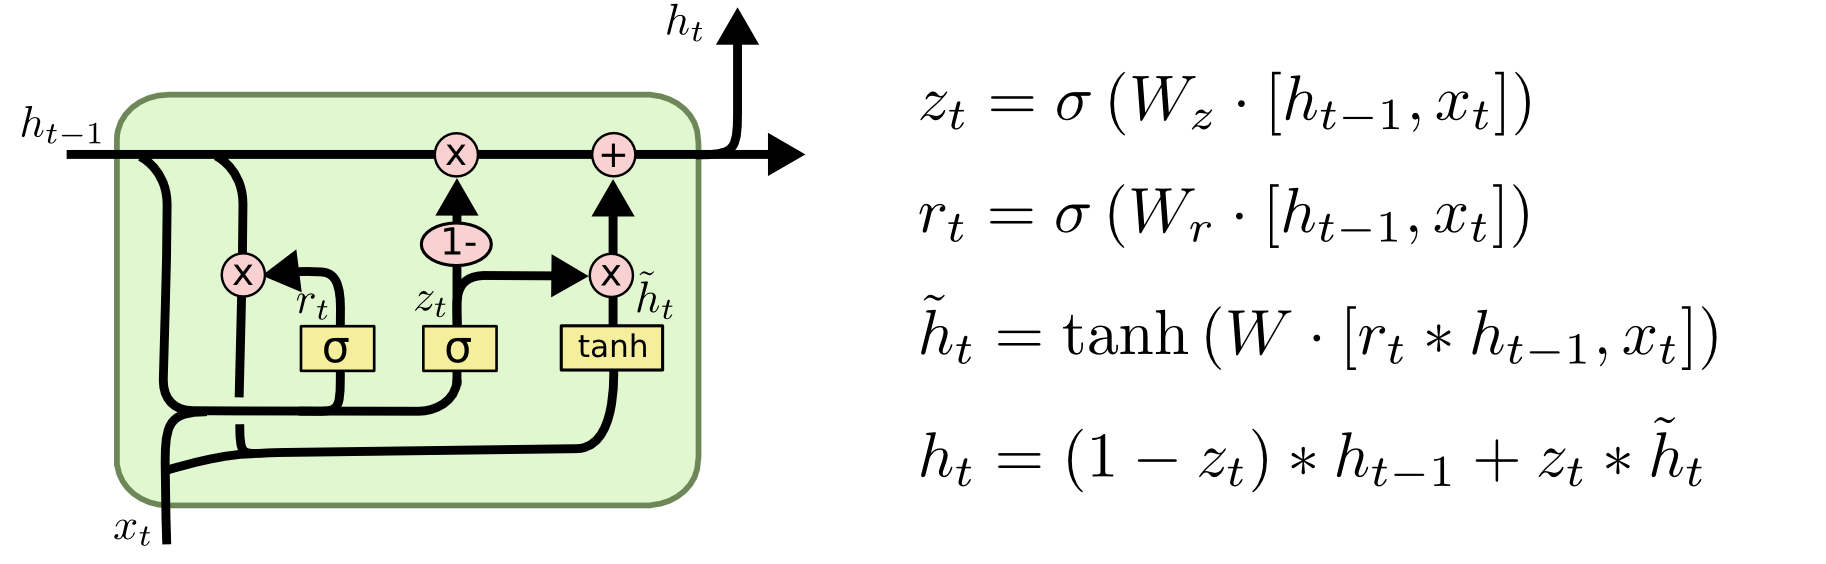
\includegraphics[height=45mm]{img/GRU.png}
	\end{figure}
	
	\clearpage
 	
	\section{Задача машинного перевода}
	
	Машинный перевод (MT) - это важная задача, направленная на перевод предложений на естественном языке с помощью компьютеров. Ранний подход к машинному переводу в значительной степени опирается на разработанные вручную правила перевода и лингвистические знания. Поскольку естественные языки по своей сути сложны, трудно охватить все языковые нарушения правилами ручного перевода. С появлением крупномасштабных параллельных корпусов все большее внимание привлекают основанные на данных подходы, которые извлекают лингвистическую информацию из данных.
	
	Нейронный машинный перевод (NMT) - это радикальный отход от предыдущих подходов к машинному переводу. С одной стороны, NMT использует непрерывные представления вместо дискретных символьных представлений. С другой стороны, NMT использует единую большую нейронную сеть для моделирования всего процесса перевода, избавляя от необходимости чрезмерного проектирования функций. Помимо своей простоты, NMT добился высочайшей производительности на различных языковых парах. На практике же NMT также становится ключевой технологией многих коммерческих систем.
	
	В качестве подхода к машинному переводу, основанного на данных, NMT использует вероятностную структуру. С математической точки зрения, цель NMT состоит в том, чтобы оценить неизвестное условное распределение $P(y|x)$ с учетом набора данных $D$, где $x$ и $y$ - случайные величины, представляющие исходный ввод и целевой вывод соответственно. Учитывая такую постановку задачи необходимо ответить на три основных вопроса:
	
	\begin{itemize}
		\item \textit{Моделирование}: Как спроектировать нейронные сети для моделирования условного распределения? 
		\item \textit{Вывод}: Учитывая входные данные источника, как сгенерировать предложение перевода из модели NMT?
		\item \textit{Обучение}: Как эффективно узнать параметры NMT из данных?
	\end{itemize}
    
    \subsection{Моделирование}
    
    Переводить можно последовательность можно на разных уровнях. В качестве единицы перевода можно взять документ, абзац или предложение. В данной работе основной единицей будет являться предложение. Благодаря такому уточнению, модель NMT можно рассматривать как модель sequence-to-sequence. 
    
    На вход подается предложение $x = {x_1, x_2, ... , x_T}$ и целевое предложение $y = {y_1, x_2, ... , y_T}$. Используя цепное правило, условное распределение может быть разложено на множители слева направо как:
    
    $$
        P(y|x = \prod\limits_{t = 1}^{T} P(y_t | y_0, y_1, ..., y_{t-1}, x_1, x_2, ..., x_S))
    $$
    
    Модели NMT, которые соответствуют данному условному распределению упоминается как авторегрессионная модель (\cite{3}, \cite{5}), поскольку прогноз на временном шаге $t - 1$ принимается в качестве входных данных на временном шаге $t$.
    
    Почти все модели нейронного машинного перевода используют структуру Encoder-Decoder. Структура энкодера-декодера состоит из четырех основных компонентов: уровней Embedding, сетей Encoder и Decoder и уровня Classification.
    
    Для однозначности конца и начала предложения в имеющуюся последовательность используются токены начала последовательности (<sos> - start of sequence) и конеца последовательности (<eos> - end of sequence). 
    
    \begin{figure}[ht!]
		\centering
		\captionsetup{justification=centering}
		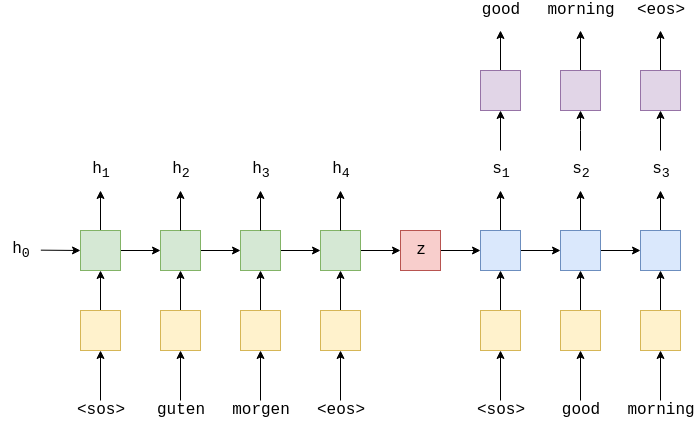
\includegraphics[height=90mm]{img/encoder-decoder-img-1.png}
		\caption{Encoder-Decoder Seq2Seq модель}
	\end{figure}
	
	Слой встраивания воплощает в себе концепцию непрерывного представления. Он отображает дискретный символ $x_t$ в непрерывный вектор $x_t \in \mathbb{R}^d$, где $d$ - размерность вектора. Затем эмбеддинг загружаются в более поздние слои для более детализированного извлечения объектов.
	
	Сеть энкодера отображает исходный эмбеддинг в скрытое состояние. Энкодер должен уметь моделировать порядок и сложные зависимости, которые существовали в исходном языке. Рекуррентные нейронные сети являются подходящим выбором для моделирования последовательностей переменной длины. Опишем RNNs вычисления, выполняемые в энкодере, как:
	
	$$
	    h_t = EncoderRNN(x_t, h_{t-1})
	$$
	
	В данном контексте под RNN может подразумеваться любая рекуррентная сеть. Например: LSTM или GRU.

	На каждом шаге итеративно применяя функцию перехода состояния $EncoderRNN$ к входной последовательности, можно использовать скрытое состояние $h_S$ в качестве представления для всего исходного предложения, а затем передать его в декодер.
	
	Декодер в свою же очередь можно рассматривать как языковую модель, обусловленную $h_S$. Сеть декодера извлекает необходимую информацию из выходных данных энкодера, а также моделирует зависимости на больших расстояниях между целевыми словами. Учитывая начальный элемент последовательности $y_0 = <sos>$ и скрытое состояние $s_0=h_S$, декодер RNN сжимает историю декодирования ${y_0, y_1, ... ,y_{t−1}}$ в вектор состояния $s_t \in \mathbb{R}^d$:
	
	$$
	    s_t = DecoderRNN(y_{t-1}, s_{t-1})
	$$
	
	Слой классификации предсказывает распределение целевых токенов. Классификация обычно представляет из себя линейный слой с функцией активации softmax. Предполагая, что словарный запас целевого языка равен $V$, а $|V|$ - это размер словарного запаса. Учитывая выходной сигнал декодера $s_t \in \mathbb{R}^d$, слой классификации сначала сопоставляет $h$ вектору $z$ в словарном пространстве $|V|$ с линейным отображением. Затем используется функция $softmax$, чтобы гарантировать, что выходной вектор является допустимой вероятностью:
	
	$$
	    sotfmax(z) = \frac{exp(z)}{\sum_{i = 1}^{|V|}exp(z_i)}
	$$
	
	где используем $z_i$ является обозначения $i$-го компонента в $z$.
	
	\subsection{Вывод}
	
	Учитывая модель NMT и входную последовательность $X$, то, вопрос как сгенерировать перевод из модели, является важной проблемой. В идеале хотелось бы найти целевую последоавтельность $y$, которое максимизирует прогноз модели $P(y|x=X;\theta)$ в качестве перевода. Однако из-за непомерно большого пространства поиска найти перевод с наибольшей вероятностью нецелесообразно. Поэтому NMT обычно использует локальные алгоритмы поиска, такие как жадный поиск или Beam search, для поиска наилучшего перевода.
	
	Beam search - это классический алгоритм локального поиска, который широко используется в NMT. Алгоритм Beam search отслеживает $k$ состояний на этапе вывода. Каждое состояние представляет собой кортеж $(y_0, y_1, ..., y_t, v)$, где $y_0, y_1, y_2, ..., y_t$ является кандидатом на перевод, а $v$ - логарифмическая вероятность кандидата. На каждом шаге генерируются все преемники всех $k$ состояний, но выбираются только верхние $k$ преемников. Алгоритм обычно завершается, когда шаг превышает заранее определенное значение или найдено $k$ полных преобразований. Следует отметить, что поиск по лучу превратится в жадный поиск, если $k = 1$.
	
	\begin{figure}[ht!]
		\centering
		\captionsetup{justification=centering}
		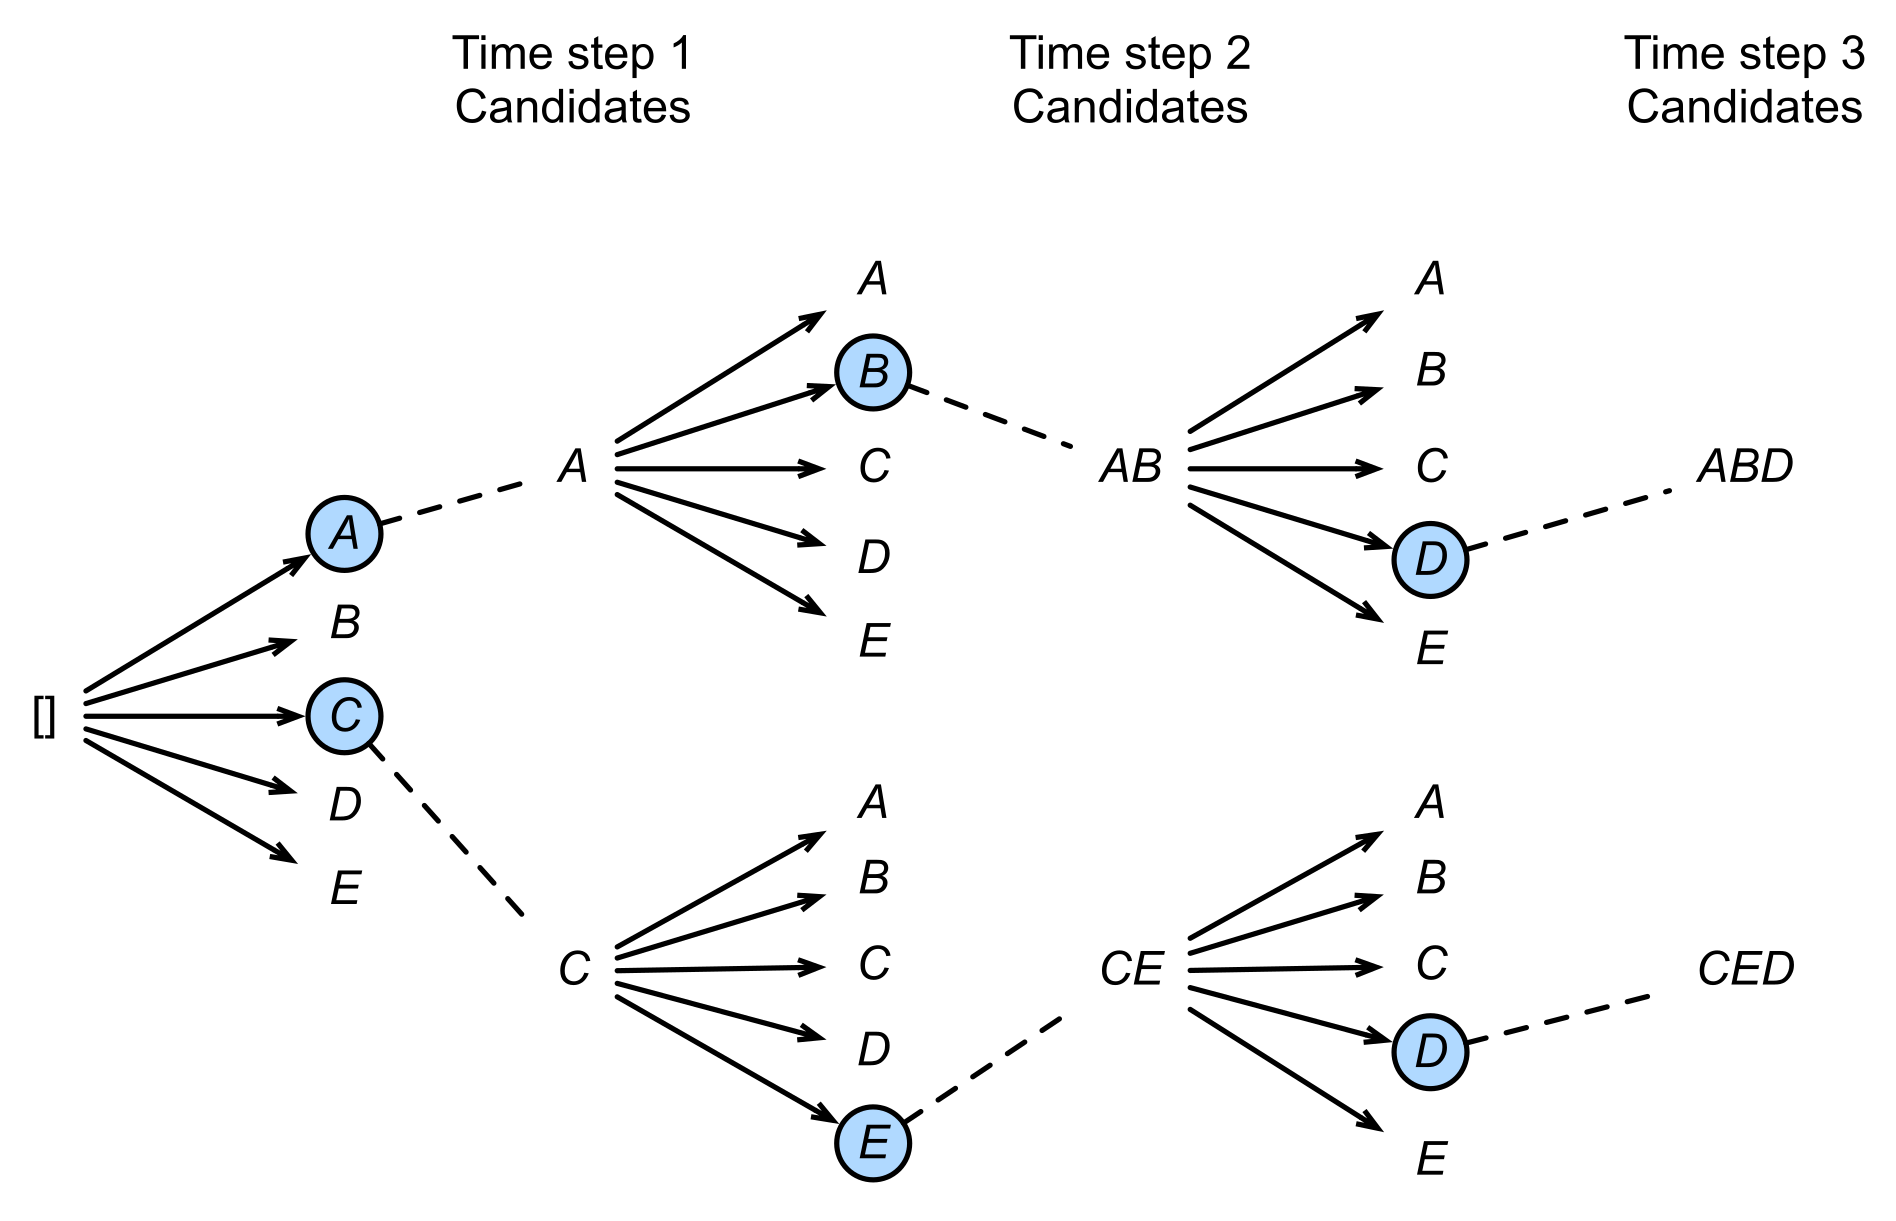
\includegraphics[height=90mm]{img/beam-search.png}
		\caption{Схема алгоритма Beam Search}
	\end{figure}
	
	
	\subsection{Обучение модели}
	
	NMT обычно использует максимальное логарифмическое правдоподобие (MLE) в качестве целевой функции обучения, которая является обычно используемым методом оценки параметров распределения вероятностей. Формально, учитывая обучающий набор $ \mathcal{D} = \{\textlangle x(s), y(s) \textrangle\}_{s=1}^S $, целью обучения является поиск набора параметров модели, которые максимизируют логарифмическую вероятность на обучающем наборе:
	
	$$
	    \hat{\theta}_{MLE} = argmax(\mathscr{L}(\theta)),
	$$

    где логарифмическая вероятность определяется как:
    
    $$
      \mathscr{L(\theta)=\sum_{s=1}^S log(P(y^{(s)}|x^{(s)};\theta))}  
    $$
    
    Благодаря алгоритму обратного распространения ошибки можно эффективно вычислить градиент $\mathscr{L}$ относительно $\theta$. При обучении моделей NMT обычно используется алгоритм стохастического градиентного поиска (SGD). Вместо вычисления градиентов на полном обучающем наборе SGD вычисляет функцию потерь и градиенты на мини-наборе обучающего набора. Простой оптимизатор SGD обновляет параметры модели NMT с помощью следующего правила:
    
    $$
        \theta \leftarrow \theta - \alpha \nabla \mathscr{L}(\theta)
    $$
    
    где $\alpha$ - скорость обучения. При правильно выбранной скорости обучения параметры NMT гарантированно сходятся к локальному оптимуму. На практике вместо обычного оптимизатора SGD обнаруживается, что адаптивные оптимизаторы скорости обучения, такие как Adam \cite{14}, значительно сокращают время обучения.
	
	\subsection{Оценка модели}
	
	Само собой итоговое модели нужно как-то проверить на их состоятельность. Почему нельзя просто оценить потери/точность итоговой системы на интересующей нас задаче?
	
	На самом деле, можно использовать два различных подхода для оценки и сравнения языковых моделей:
	
	\begin{enumerate}
	    \item \textit{Внешняя оценка}. В данном случае применяется оценивание модели путём решения с её помощи задачи, на которую она рассчитана (в нашем случае задачи машинного перевода), и анализ итоговых показателей потерь/точности. Это лучший подход к оцениванию моделей, так как это — единственный способ реально оценить то, как разные модели справляются с интересующей нас задачей. Но реализация этого подхода может потребовать больших вычислительных мощностей, его применение может оказаться медленным, так как для этого нужно обучение всей анализируемой системы.
	    \item \textit{Внутренняя оценка}. Тут же используется подход, предусматривающий поиск некоей метрики для оценки самих языковых моделей, без учёта конкретных задач, для решения которых их планируется использовать. Хотя внутренняя оценка моделей не так «хороша», как внешняя, если речь идёт об итоговой оценке модели, она являет собой полезное средство для быстрого сравнения моделей.
	\end{enumerate}
	
	В данной работе в качестве метрики используется BLEU (Bilingual Evaluation Understudy) на данный момент самая популярная в современной оценке МП. Позволяет учитывать не только точность перевода отдельных слов, но и цепочек слов (N-граммы).

    Метрика BLEU была разработана сотрудниками компании IBM и является одной из самых простых в использовании метрик оценки машинного перевода. Алгоритм BLEU оценивает качество перевода по шкале от 0 до 100 на основании сравнения машинного перевода с человеческим и поиска общих слов и фраз. Основная идея разработчиков метрики состоит в том, что чем лучше машинный перевод, тем больше он должен быть похож на человеческий.
    
    Лучше На маленьком объёме текста метрика зачастую обнуляется из-за отсутствия совпадающих 4-грамм и работает некорректно. Существуют также доработанные варианты метрики, которые подходят для сравнения на уровне предложения.е всего такая метрика работает не на уровне предложений, а на уровне большого текст
    
    Для большего понимания как работает данная метрика, разберем пару примеров из статьи \cite{15}.
    
    Пример плохого машинного перевода:
    \begin{table}[h]
        \centering
        \begin{tabular}{|l|c|c|c|c|c|c|c|}
        \hline
        \textbf{Кандидат}  & the   & the & the & the & the & the & the \\ \hline
        \textbf{Ссылка №1} & the   & cat & is  & on  & the & mat &     \\ \hline
        \textbf{Ссылка №2} & there & is  & a   & cat & on  & the & mat \\ \hline
        \end{tabular}
    \end{table}
    
    Из семи слов в переводе-кандидате все они фигурируют в ссылочных переводах. Таким образом, тексту-кандидату присваивается точность однограммы, равная:
    
    $$
        P = \frac{m}{w_t} = \frac{7}{7} = 1
    $$
    
    где $m$ - количество слов из кандидата, найденных в ссылке, а $w_t$ - общее количество слов в кандидате. Это идеальная оценка, несмотря на то, что приведенный выше перевод-кандидат сохраняет мало содержания любой из ссылок.
    
    Модификация, которую вносит BLEU, довольно проста. Для каждого слова в переводе-кандидате алгоритм принимает его максимальное общее количество, $m_{max}$, в любом из эталонных переводов. В приведенном выше примере слово \textit{the} появляется дважды в ссылке №1 и один раз в ссылке №2. Таким образом $m_{max}=2$.
    
    Для перевода-кандидата количество $m_{w}$ каждого слова обрезается до максимального значения $m_{max}$ для этого слова. В этом случае \textit{the} имеет $m_{w}=7$ и $m_{max}=2$, таким образом, $m_{w}$ обрезается до $2$. Эти отсеченные подсчеты $m_{w}$ затем суммируются по всем отдельным словам в кандидате. Затем эта сумма делится на общее количество униграмм в переводе кандидата. В приведенном выше примере измененный показатель точности униграмм будет равен:
    
    $$
        P = \frac{2}{7}
    $$
    
    Однако на практике использование отдельных слов в качестве единицы сравнения не является оптимальным. Вместо этого BLEU вычисляет ту же самую модифицированную метрику точности, используя n-граммы. Было обнаружено, что длина, которая имеет "самую высокую корреляцию с одноязычными человеческими суждениями", равна четырем. Установлено, что оценки униграмм учитывают адекватность перевода и то, сколько информации сохраняется. Более длинные оценки по n-граммам учитывают беглость перевода или то, в какой степени.
    
    Сравнение показателей для кандидата \textit{the the cat}:
    
    \begin{table}[h]
        \centering
        \begin{tabular}{|l|l|l|}
        \hline
        Модель                    & Набор граммов    & Оценка \\ \hline
        Униграмм                  & the, the, cat    & $\frac{1+1+1}{3} = 1$      \\ \hline
        Сгруппированная Униграмма & the*2, cat*1     & $\frac{1+1}{2+1} = \frac{2}{3}$      \\ \hline
        Биграмм                   & the the, the cat & $\frac{0+1}{2} = \frac{1}{2}$       \\ \hline
        \end{tabular}
    \end{table}
    
    Примером возможного перевода для тех же ссылок, что и выше, может быть:
    
    \ \ \ \ \textit{the cat}
    
    В этом примере измененная точность однограммы будет равна,
    
    $$
        P = \frac{1}{2} + \frac{1}{2} = \frac{2}{2}
    $$
    
    поскольку слово \textit{the} и слово \textit{cat} появляются в кандидате по одному разу, а общее количество слов равно двум. Измененная точность биграммы будет равна $\frac{1}{1}$ в качестве биграммы \textit{cat} появляется один раз в кандидате. Было отмечено, что точность обычно сочетается с отзывом, чтобы преодолеть эту проблему, так как отзыв униграмм в этом примере будет $\frac{3}{6}$ или $\frac{2}{7}$. Проблема заключается в том, что, поскольку существует несколько ссылочных переводов, плохой перевод может легко вызвать завышенную отзывчивость, например, перевод, который состоял из всех слов в каждой из ссылок.
	\clearpage
	
	\section{Сбор данных}
	
	Краеугольным камнем в машинном обучении является качество данных. В нашем случае выходной результат, буквально, в большей степени зависит от количества и качества данных.
	
	В работе было применено несколько дата-сетов для проверки реализации модели машинного перевода.
	
	\begin{enumerate}
		\item \textit{RUS $\shortrightarrow$ ENG} - Дата-сет предложений с переводом с русского языка на английский.
		\begin{enumerate}
			\item ManyThings.org - Двуязычные Пары предложений, разделенные табуляцией. 
			Это выбранные пары предложений из проекта Tatoeba. \\ 
			\url{http://www.manythings.org/anki/}
		\end{enumerate}
		\item \textit{RUS $\shortrightarrow$ OSS} - Дата-сет предложений с пользовательским переводом с русского языка на осетинский.
		Кусочно собран с разных ресурсов, таких как:
		\begin{enumerate}
			 \item Проект \textit{Tatoeba} - обширная база данных предложений и их переводов, постоянно пополняющаяся усилиями тясяч добровольных участников. \\ \url{https://tatoeba.org/ru/downloads}
			 \item Проект \textit{Биоингвӕтӕ} - Билингвы подготовлены для чтения с помощью электронных словарей программы Lingvo. \\ \url{https://ironau.ru/bilingva/index.htm}
			 \item Ф.М. Таказов - Краткий русско-осетинский разговорник. \\ \url{https://ironau.ru/takazov/phrasebook2.htm}
			 \item Ф.М. Таказов - Самоучитель осетинского языка. \\ \url{https://ironau.ru/takazov/index.htm}
 		\end{enumerate}
	\end{enumerate}

    \newpage

	\section{Релазизация модели NMT-Seq2Seq в TensorFlow}
	
	\subsection{Подготовка даных}
	
	Загрузим необходимые библиотеки.
	
	\begin{lstlisting}[language=iPython]
import matplotlib.pyplot as plt

import re, os, time, random
import pandas as pd
import numpy as np

import tensorflow as tf
import pickle as pkl

from sklearn.model_selection import train_test_split
from keras.preprocessing.text import Tokenizer
from keras.models import model_from_json
from keras.models import Model, load_model
from keras.layers import LSTM, GRU, Input, Dense, Embedding
from keras.preprocessing.sequence import pad_sequences

from prettytable import PrettyTable
from nltk.translate.bleu_score import sentence_bleu \end{lstlisting}

    \begin{figure}[ht!]
		\centering
		\captionsetup{justification=centering}
		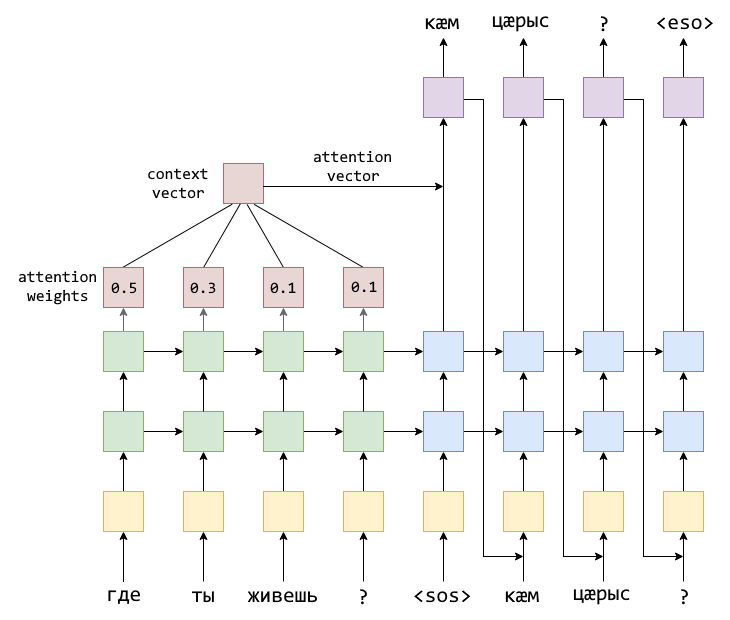
\includegraphics[height=140mm]{img/Model.png}
		\caption{Модель}
	\end{figure}
    \clearpage
	
	\addcontentsline{toc}{section}{Список используемой литературы}
	
	\begin{thebibliography}{}
		\bibitem{1}  Michael I. Jordan	-	Serial Order: A Parallel Distributed Processing Approach; 1986. 
		
		\url{https://cseweb.ucsd.edu/~gary/PAPER-SUGGESTIONS/Jordan-TR-8604-OCRed.pdf}
		
		\bibitem{2}  S. Hochreiter, J. Schmidhuber	-	Long Short-Term Memory; 1997.
		
		\url{https://www.researchgate.net/publication/13853244_Long_Short-term_Memory}
		
		\bibitem{3}  Junyoung Chung, Caglar Gulcehre, KyungHyun Cho, Yoshua Bengio	-	Empirical Evaluation of Gated Recurrent Neural Networks on Sequence Modeling; 2014.
		
		\url{https://www.researchgate.net/publication/269416998_Empirical_Evaluation_of_Gated_Recurrent_Neural_Networks_on_Sequence_Modeling}
		
		\bibitem{4} J. Elman	-	Finding Structure in Time; 1990.
		
		\url{http://psych.colorado.edu/~kimlab/Elman1990.pdf}
		
		\bibitem{5} Ilya Sutskever	-	Training recurrent neural networks; 2013.
		
		\url{https://www.cs.utoronto.ca/~ilya/pubs/ilya_sutskever_phd_thesis.pdf}
		
		\bibitem{6} Ян Гудфеллоу, Иошуа Бенджио, Аарон Курвилль	-	Глубокое обучение; М.: ДМК Пресс, 2018 - 652c. 
		
		\bibitem{7} С. Николенко, А. Кадурин, Е. Архангельская	-	Глубокое обучение;  СПб.: Питер, 2018 - 480c.
		
		\bibitem{8} Alex Sherstinsky	-	Fundamentals of Recurrent Neural Network (RNN) and Long Short-Term Memory (LSTM) Network; 2018.
		
		\url{https://www.researchgate.net/publication/326988050_Fundamentals_of_Recurrent_Neural_Network_RNN_and_Long_Short-Term_Memory_LSTM_Network}
		
		\bibitem{9} Zachary Chase Lipton	-	A Critical Review of Recurrent Neural Networks for Sequence Learning; 2015.
		
		\url{https://www.researchgate.net/publication/277603865_A_Critical_Review_of_Recurrent_Neural_Networks_for_Sequence_Learning}
		
		\bibitem{10} Ri Wang, Maysum Panju, Mahmood Reza Gohari -   Classification-based RNN machine translation using GRUs; 2017
		
		\url{https://www.researchgate.net/publication/315570520_Classification-based_RNN_machine_translation_using_GRUs}
		
		\bibitem{11} Tomohiro Fujita, Zhiwei Luo, Changqin Quan, Kohei Mori - Simplification of RNN and Its Performance Evaluation in Machine Translation; 2020
		
		\url{https://www.jstage.jst.go.jp/article/iscie/33/10/33_267/_pdf/-char/en}
		
		\bibitem{12} Sainik Kumar Mahata, Dipankar Das and Sivaji Bandyopadhyay -  MTIL2017: Machine Translation Using Recurrent Neural Network on Statistical Machine Translation; 2018
		
		\url{https://www.researchgate.net/publication/325456613_MTIL2017_Machine_Translation_Using_Recurrent_Neural_Network_on_Statistical_Machine_Translation}
		
		\bibitem{13} Zhixing Tan, Shuo Wang, Yang Zonghan, Gang Chen - Neural Machine Translation: A Review of Methods, Resources, and Tools; 2020
		
		\url{https://www.researchgate.net/publication/348079690_Neural_Machine_Translation_A_Review_of_Methods_Resources_and_Tools}
		
		\bibitem{14} Timothy Mayer, Ate Poortinga, Biplov Bhandari, Andrea P. Nicolau, Kel Markert, Nyein Soe Thwal, Amanda Markert, Arjen Haag, John Kilbrideh, Farrukh Chishtie, Amit Wadhwai, Nicholas Clintonj, David Saah - Deep Learning approach for Sentinel-1 Surface Water Mapping leveraging Google Earth Engine; 2021
		
		\url{https://www.researchgate.net/publication/355005296_Deep_Learning_approach_for_Sentinel-1_Surface_Water_Mapping_leveraging_Google_Earth_Engine}
		
		\bibitem{15} Kishore Papineni, Salim Roukos, Todd Ward, Wei-Jing Zhu - BLEU: a Method for Automatic Evaluation of Machine Translation; 2002
		
		\url{https://www.researchgate.net/publication/2588204_BLEU_a_Method_for_Automatic_Evaluation_of_Machine_Translation}
	\end{thebibliography}
\end{document}


% \begin{lstlisting}[language=iPython]

% \end{lstlisting}